\newpage
\begin{center}
  \textbf{\large 1. ТЕОРЕТИЧЕСКАЯ ЧАСТЬ}
\end{center}
\refstepcounter{chapter}
\addcontentsline{toc}{chapter}{1. ТЕОРЕТИЧЕСКАЯ ЧАСТЬ}

\addcontentsline{toc}{subsubsection}{Потенциалы оценочнной функции}

\section{Потенциалы оценочной функции}

Электростатические взаимодействия между мозаично распределенными на поверхности белка электрическими зарядами являются основным фактором, определяющим специфичность взаимодействий в белковых комплексах\cite{chrushev}. Поэтому при разработке оценочной функции для моделирования компонент в~виде <<твёрдых>> тел без конформационных изменений возможно опустить оценку ковалентных и~внутримолекулярных нековалетных взаимодействий. В исследовании для описания межмолекулярных взаимодействий используются общепринятые эмпирические парные потенциалы Леннард--Джонса и Кулона. Энергия растворителя вычисляется в рамках модели неявного растворителя EEF1 \cite{eef1}.

Поскольку разработка оценочной функции невозможна без учёта физических параметров атомов белка и растворителя в работе использовались данные широко распространённого силового поля CHARMM36\cite{brooks}.


\subsection{Потенциал Кулона}


Потенциал Кулона в биоинформатике относится к электростатическому потенциалу, возникающему из взаимодействия заряженных частиц, таких как ионы и заряженные аминокислоты в биологических молекулах. Этот потенциал играет важную роль в стабилизации структуры белков и их функционировании, а также во взаимодействии между биомолекулами, такими как белки, нуклеиновые кислоты и мембраны.

В биоинформатике потенциал Кулона используется для моделирования и предсказания структуры и функции биомолекул, а также для анализа их взаимодействий. Например, при моделировании структуры белка учёт электростатических взаимодействий между заряженными аминокислотами может помочь определить стабильные конформации и предсказать функциональные сайты белка.

Для расчёта потенциала Кулона в биоинформатике используются различные методы, такие как численные методы, аппроксимации и теория возмущений. Один из наиболее распространённых подходов - методы решения уравнения Пуассона-Больцмана, которое описывает распределение зарядов и потенциалов в системе с учётом диэлектрических свойств окружающей среды.

Важно отметить, что потенциал Кулона является только одним из аспектов, которые нужно учитывать при анализе биомолекул. Другие факторы, такие как гидрофобные взаимодействия, ван-дер-ваальсовы силы и водородные связи, также играют ключевую роль в структуре и функции биомолекул.

Потенциал Кулона вычисляется по следующей формуле \ref{kp} 

\begin{equation}
	E_{c}=\sum_{i,j}\left({\frac{1}{4 \pi \varepsilon_{r}}} \frac{q_{i}q_{j}}{d_{ij}} \left[ \frac{d^{2}_{ij}}{k^{2}} - \frac{2 d_{ij}}{k} + 1 \right]\right),
	\label{kp}
\end{equation}
где $d_{ij}$ -- евклидово расстояние между центрами атомов, $q_{i}$ и~$q_{j}$ --~фиксированные частичные атомные заряды в~рассматриваемой паре атомов, $\varepsilon_{r}$ --~диэлектрическая константа. Атомные заряды получены с~помощью программы PDB2PQR~\cite{pdb2pqr}. Вместо первой дроби при вычислениях используется константа, применяемая в~силовом поле~CHARMM:~$332.0716$~ккал${\cdot}$\AA${\cdot}e^{-2}/$моль. Последний множитель с~коэффициентом~$k=14$\AA \ определяет радиус сферы взаимодействия, для $d_{ij} > k$ вычисления не производятся.

% TODO: нормально расставить ссылки
%И1  \cite{ci500731a}

%И2  \cite{biom10071056}

%И3  \cite{Voter}

%И4  \cite{chrushev}

%И5  \cite{Voter}

%И6  \cite{brooks}

%И7  \cite{wu}

%И8  \cite{rate, eef1}

%И9 	\cite{vcs}

%И10 \cite{pdb2pqr}


\subsection{Потенциал Леннард-Джонса}

Потенциал Леннард-Джонса в биоинформатике используется для моделирования межатомных взаимодействий, особенно ван-дер-ваальсовых сил, которые играют важную роль в стабилизации структуры и функции биомолекул, таких как белки и нуклеиновые кислоты.

Потенциал Леннард-Джонса представляет собой математическую функцию, которая описывает силы притяжения и отталкивания между атомами на основе их расстояния. Он состоит из двух компонентов: дисперсионного (притягательного) и репульсивного (отталкивающего) членов. Дисперсионный член возникает из квантовых флуктуаций электронных облаков атомов, в то время как репульсивный член связан с запретом на проникновение электронных облаков друг в друга из-за принципа запрета Паули.

В биоинформатике потенциал Леннард-Джонса используется для моделирования структуры и динамики биомолекул, таких как белки, нуклеиновые кислоты и липидные мембраны. Он позволяет учесть межатомные взаимодействия, которые влияют на стабильность и функциональность этих молекул. Например, при моделировании структуры белка учет ван-дер-ваальсовых сил, описываемых потенциалом Леннард-Джонса, может помочь определить стабильные конформации и предсказать функциональные сайты белка.

Потенциал Леннард-Джонса также используется в молекулярном докинге для предсказания структуры комплексов между биомолекулами, такими как белки и лиганды или белки и нуклеиновые кислоты. В этом контексте потенциал Леннард-Джонса помогает определить оптимальные конформации и оценить энергию связывания между молекулами.

Важно отметить, что потенциал Леннард-Джонса является только одним из аспектов, которые нужно учитывать при анализе биомолекул. Другие факторы, такие как электростатические взаимодействия, гидрофобные силы и водородные связи, также играют ключевую роль в структуре и функции биомолекул.

Потенциал Леннард-Джонса вычисляется по следующей формуле \ref{ld}

\begin{equation}
	\displaystyle E_{v}=\sum _{i,j}\left(\varepsilon_{ij}\left[\left({\frac {R_{ij}}{d_{ij}}}\right)^{12}-2\left({\frac {R_{ij}}{d_{ij}}}\right)^{6}\right]\right), \ R_{ij} = \frac{R_{i}}{2} + \frac{R_{j}}{2}, \ \varepsilon_{ij} = \sqrt{\varepsilon_{i} \varepsilon_{j}},
	\label{ld}
\end{equation}
где $d_{ij}$ -- евклидово расстояние между центрами атомов, $R_{i}$ и~$R_{i}$ -- расстояния, на которых значение потенциала становится равным нулю, $\varepsilon_{i}$ и~$\varepsilon_{j}$ -- глубины потенциальных ям. Указанные параметры получены из файла топологии для соответствующих типов атомов в рассматриваемой паре атомов с индексами $i$ и~$j$.

Необходимо отметить, что потенциал Леннард--Джонса в классическом виде \ref{ld} не используется в силовом поле CHARMM. Для описания сил Ван-дер-Ваальса используется двойной экспоненциальный потенциал \cite{wu}. Он позволяет более точно оценить энергию, поскольку использует отдельные функции для оценки эффекта притяжения и отталкивания, а также отдельную процедуру для учета дальнодействующих взаимодействий.

\subsection{Неявный растворитель}


Знание эффективной энергетической гиперповерхности биологических макромолекул в растворе имеет фундаментальное значение для понимания их свойств. Эффективная энергия (потенциал средней силы) для данной конформации макромолекулы представляет собой свободную энергию системы, состоящей из макромолекулы и растворителя, усредненную по всем степеням свободы растворителя при заданной температуре. Она состоит из внутримолекулярной энергии (энергия макромолекулы в вакууме) и энергии свободного растворения (свободная энергия переноса макромолекулы из газовой фазы в раствор). Общая свободная энергия системы макромолекула-растворитель в данной области гиперповерхности является суммой средней эффективной энергии и конфигурационной энтропии. В физиологических условиях обычно предполагается, что белки стабильны в окрестности глобального минимума (родной конформации), несмотря на большой прирост конфигурационной энтропии в денатурированном состоянии. Это называется "термодинамической гипотезой" стабильности белка, и имеющиеся данные свидетельствуют о ее справедливости для большинства малых однодоменных белков. Даже там, где эргодичность, кажется, нарушается, родное состояние должно соответствовать глубокому минимуму на эффективной энергетической гиперповерхности, который отделен от глобального минимума барьерами, слишком высокими для преодоления на экспериментальных временных шкалах. Теоретические прогнозы структуры белка из последовательности аминокислот и анализ механизма складывания требуют знания эффективной энергетической гиперповерхности и метода эффективного поиска конформационного пространства для определения расположения минимумов.

Всеатомные силовые поля, используемые в молекулярной механике и динамике симуляций макромолекул, дают энгию белка в вакууме. Только введя явный растворитель и проведя симуляции, показывающие как макромолекулу, так и растворитель, можно учитывать эффекты соляции. Из результатов симуляций и теоретических соображений ясно, что эффективная гиперповерхность энергии, включающая растворитель, значительно отличается от внутримолекулярной гиперповерхности энергии. Хотя внутримолекулярная гиперповерхность энергии часто имеет глубокий минимум около нативной конформации, она может иметь другие равно глубокие или более глубокие минимумы в отдаленных областях пространства конформации. Это может возникнуть из-за ряда эффектов. Например, взаимодействия полярных-неполярных групп в газовой фазе энергетически выгодны так же, как и полярные-неполярные взаимодействия. Однако в воде полярно-неполярные взаимодействия эффективно отталкивают из-за высокого штрафа за десольватацию полярной группы. Кроме того, гидрофобная гидратация делает эффективные взаимействия между неполярными группами в воде сильнее, чем в газовой фазе. Таким образом, вода способствует стабилизации нативного состояния с зарытыми неполярными группами и помогает гарантировать его уникальность. Взаимодействия противоположных зарядов менее стабилизирующие в воде, чем в вакууме. Таким образом, проблемы, связанные с складыванием и стабильностью белков, не могут быть решены без учета соляции.

Хотя за последние 40 лет был сделан значительный прогресс в статистической теории жидкостей, все еще отсутствуют простые и точные модели водной соляции. В настоящее время наиболее надежным методом учета соляции является симуляция белка в присутствии явных молекул воды. Однако этот подход связан с большими вычислительными затратами, и большая часть времени компьютера в таких симуляциях уходит на расчет взаимодействий растворителя-растворителя. Например в симуциях денатурации барназа система состояла из 1100 атомов белка и около 9000 атомов растворителя. Включение такого большого количества атомов растворителя ставит серьезные ограничения на тип проблем, которые можно изучать. Например, хотя динамику нативных состояний можно эффективно симулировать с помощью явных моделей растворителя, симуляции раскладки (и раскладанных состояний) на временных масштабах, необходимых для выборки достаточного количества различных начальных состояний для получения значимых сходимых результатов, пока что невозможны, за исключением, возможно, маленьких пептидов.

Еще одним ограничем симуляций явной соляции является то, что разница свободной энергии не получается прямым способом. Например, точное моделирование воды в нативной и неправильно свернутой структурах не показывает, какая из них имеет наименьшую свободную энергию. Требуется особая симуляция, включающая обратимый переход от одной конформации к другой или выборка по зонтику, чтобы можно было рассчитать необходимые различия в свободной энергии. Такие симуляции были проведены главным образом для малых молекул, таких как бутан, дипептиды и другие маленькие пептиды. Недавно потенциал средней силы для маленького белка относительно радиуса инерции в качестве параметра порядка был рассчитан с явным растворителем; для этой симуляции потребовалось 450 часов процессорного времени на 64-узловом Т3Е-суперкомпьютере (эквивалент 4 месяцам на стандартной рабочей станции). Таким образом, использованте этого подхода для изучения деталей сложенных и раскладанных состояний ряда белков, а также многих других проблем текущего интереса, все еще невозможно. 

Чтобы преодолеть ограничения вакуумных расчетов, с одной стороны, и явных симуляций растворителя, с другой, было разработано множество невных моделей соляции для белков, которые объединяют эмпирическое силовое поле для внутримолекулярных взаимодействий в вакууме с коррекцией сольвации. Последняя получается путем рассмотрения переноса всего белка или соответствующих составных групп из газовой фазы в воду. Очень простая модель использовала потенальную энергию CHARMM и коррекцию соляции на основе площади поверхности атома; были включены пять различных типов атомов. Та же модель соляции была объединена с силовым полем AMBER Шиффера. Фратернали и ван Гунстерен предложили еще более простую модель для использования в молекурной динамике (MD); эта модель также основана на доступных поверхностях и использует только два параметра - один для неполярных и один для полярных групп.

Хотя вышеупомянутые модели оценивают эффект соляции в терминах площади поверхности, нет фундаментального теоретического обоснования для этого выбора. Модель, которая не использует площадь поверхности, - это модель гидратационной оболочки. Она предполагает, что свободная энергия гидратации группы возникает из первой гидратационной оболочки и пропорциональна объему гидратационной оболочки, доступной растворителю (т.е. не занятой другими атомами растворителя). Еще один тип модели соляции основан на контактах, которые каждая группа устанавливает с другими атомами растворителя. Чем больше контактов, тем меньше величина свобной энергии соляции группы, и контакты взвешиваются в соответствии с некоторой функцией их расстояния от группы. Эта модель похожа на подходы, использованные ранее Гибсоном, Шерагой и Левиттом. Физически, модель Колонна-Чезари-Сандера похожа на модели площади поверхности, но она намного быстрее в использовании, потому что подсчет количества контактов занимает значительно меньше времени, чем даже самые эффективные аналитические методы расчета площади поверности. Кроме того, аналитические производные свободной энергии соляции могут быть легко получены для оценки сил, необходимых для минимизации энергии и молекулярной динамики. Версия этой модели была параметризована на основе свободных энергий гидратации малых молекул. Для каждой группы назначается параметр соляции. Модель была объединена с полем сил GROMOS и использована в стохастической динамической симуляции инибита трипсина поджелудочной железы крупного рогатого скота (BPTI). Было обнаружено, что полученные структуры были разумными, хотя отклонение от кристалличкой структуры было немного больше, чем в симуляциях с явной водой. 

Другой набор моделей сольватации рассматривает весь белок сразу и основан на континуальной электростатике и линеаризованном уравнении Пуассона-Больцмана. Поскольку численные решения уравнения Пуассона-Больцмана дороги, были предложены полуаналитические или аналитические приближения. Стилл ввел простое обобщение формулы Борна на многоатомные молекулы. Позднее обобщенное уравнение Борна было объединено с методом интегрированного поля для собственных энергий, что дало полностью аналитическую трактовку электростатических энергий и сил.38 Были сделаны приложения к ряду простых систем, и вполне вероятно, что этот подход будет использоваться более широко в будущем.

\textbf{Описание модели.}

Эффективная энергия $W(R^M)$ макромолекулы с координатами $R^M$ в решении может быть записана следующим образом

\begin{equation}
	W(R^M) = H_{intra}(R^M) + \Delta G^{slv}(R^M),
	\label{ee}
\end{equation}

где 

\begin{itemize}
	\item $H_{intra}$ -- внутримакромолекулярная энергия
	\item $\Delta G^{slv}$ -- свободная энергия растворителя
\end{itemize}

Чтобы получить данное уравнение \ref{ee}, единственное предположение состоит в том, что гамильтониан является сепарабельным; то есть это сумма терминов раствор-раствор, раствор-растворитель и растворитель-растворитель. Так обстоит дело с большинством эмпирических функций энергии, которые не включают поляризацию. Недавняя теоретическая работа по термодинамике сольватации показала, что свободная энергия сольватации $\Delta G^{slv}$ заданной конформации $R^M$ может быть записана как интеграл по окружающему пространству; то есть,

\begin{equation}
	\Delta G^{slv} = \int f(r)dr,
	\label{fe}
\end{equation}

где $f(r)$ -- плотность свободной энергии сольватации в точке $r$. Она состоит из энергии расстворенного вещества-растворителя, энергии преобразования растворителя, энтропии раствора-растворителя и энтропии преобразования растворителя. Ожидается, что плотность свободной энергии растворителя сильно зависит от расстояния. Ее величина достигает максимума вблизи состояния раствора и стремится к нулю при отдалении от этого состояния. Когда две молекулы раствора приближаются друг к другу или изменяется конформация многоатомного раствора, сольватация каждой группы изменяется из-за двух эффектов: исключение растворителя из пространства, которое занято другими группами раствора, и изменение плотности ориентационного распределения растворителя в пространстве, которое не занято раствором. Для электростатических взаимодействий собственная энергия зарядов относится к первой категори, а диэлектрическое экранирование ко второй. В представленной модели упускается второй эффект для неполнярных групп, поскольку ожидается, что он будет незначительно малым, но он частично учитывается для полярных грпп за счет использования диэлетричской проницаемости, котороая зависит от расстояния. Предполагается, что для многоатомного раствора свободную энергию сольватации можно записать как сумму групп, то есть,

\begin{equation}
	\Delta G^{slv} = \sum_i \Delta G_i^{slv},
	\label{fem}
\end{equation}

где $\Delta G_i^{slv}$ -- свободная энерегия сольватации группы $i$. Выражение \ref{fem} может быть формально получено путем рассмотрения энергии взаимодействия раствора и растворителя как суммы взаимодействия группы и растворителя и корреляционной функции раствора и растворителя как произведения корреляционных функций группы и растворителя. Принимая во внимание только эффект исключения растворителя, можно записать 

\begin{equation}
	\Delta G_i^{slv} = \Delta G_i^{ref} - \sum_j \int_{V_j} f_i(r) dr,
	\label{femws}
\end{equation}

где $\Delta G_i^{ref}$ (эталонная свободная энергия сольватации) -- свободная энергия сольватации $i$ в молекуле, выбранной подходящим образом, в которой группа $i$ практически полностью подвергается воздействию растворителя. Интеграл в выражении находится по объему $V_j$ группы $j$, а суммирование происходит по всем группам $j$ вокруг $i$. Для упрощения вычислений интеграл по $f_i(r)$ заменяется произведением $f_i(r_{ij})V_j$, то есть

\begin{equation}
	\Delta G_i^{slv} = \Delta G_i^{ref} - \sum_{j \neq 1} f_i(r_{ij}) V_j,
	\label{ufemws}
\end{equation}

где $r_{ij}$ -- расстояние между $i$ и $j$. Выражние \ref{ufemws} сообщает, что свободная энергия сольватации группы $i$ равна энергии в модельной системе $\Delta G_i^{ref}$ за исключением сольватации из-за присутствия окружающих групп. Предполагаемая плотность свободной энергии сольватации определяется функцией Гаусса.

\begin{equation}
	f_i(r) 4 \pi r^2 = \alpha_i exp(-x_i^2), x_i = \frac{r - R_i}{\lambda_i},
	\label{gf}
\end{equation}

где $R_i$ -- ван дер Ваальсов радиус $i$, равный $\frac{1}{2}$ расстояния до энергетического минимума в потенциале Леннард-Джонса, $\lambda_i$ корреляционная длинна и $\alpha_i$ -- коэффициент пропорциональности, равный

\begin{equation}
	\alpha_i = \frac{2 \Delta G_i^{free}}{\sqrt{\pi \lambda_i}},
	\label{kpr}
\end{equation}

где $\Delta G_i^{free}$ -- свободная энергия сольватации изолированной группы $i$; $\Delta G_i^{free}$ близка к $\Delta G_i^{ref}$, но не тождественно и определеяется эмпирически, требуя, чтобы свободная энергия сольватации глубоко лежащих групп равнялась нулю.


% TODO: потом убрать, если нисего отсюда не нужно
%Неявный растворитель -- это математическая модель, основанная на модели Гауссовских гидратных оболочек, которая используется для описания структуры гидратации белков и других макромолекул. Эта модель основана на предположении, что молекулы воды вблизи поверхности белка образовывают некоторую сферическую оболочку, в которой плотность молекул воды стремится к нулю. Разработчики использовали гауссовские функции, чтобы определить энергию гидратации каждого атома белка.

%Гидратная оболочка атома -- слой молекул воды, которые окружают атом и связаны с ним посредством водородных связей. То есть, гауссовские функции используются для моделирования гидратационной оболочки вокруг атомов белка, что позволяет более точно выполнить расчет энергии гидратации каждого отдельного атома.

%Модель Гауссовских гидратных оболочек предполагает, что размещение молекул воды в области гидратации с увеличением расстояния от белка может быть описано функцией Гаусса. Эта функция характеризуется средним значением и стандартным отклонением, которые определяют размеры и форму гидратной оболочки.

%Модель Гауссовских гидратных оболочек позволяет получить количественную оценку химических взаимодействий между белком и водой. В частности, эта модель используется для выявления ключевых аминокислотных остатков в белке, которые взаимодействуют с водой и играют важную роль в его структуре и функции.

%Более новые версии модели, такие как модель гидратации Майкросольвентной оболочки или модель Гижи-Шавитца, учитывают сильные динамические и корреляционные эффекты между молекулами воды и их взаимодействие с белком.

%Однако, важно понимать, что модель Гауссовских гидратных оболочек является лишь упрощенной моделью, которая не может учитывать полную динамику гидратации белка. Несмотря на это, она остается полезным инструментом для анализа структуры и функции белков в различных условиях.

%Формула неявного растворителя имеет вид:
%\[ E_s = \sum_i \Delta G_i + \sum_{i,j} \left( \frac{1}{2 \pi \sqrt{\pi}} \left[ -\Delta G_i e^{-\left( \tfrac{d_{ij} - {R_i}^{\textquotesingle}}{\lambda_i} \right)^2} - \Delta G_j e^{-\left( \tfrac{d_{ij} - {R_j}^{\textquotesingle}}{\lambda_j} \right)^2} \right] \right), \]
%где:
%\begin{itemize}
%	\item $d_{ij}$ -- евклидово расстояние между центрами атомов
%	\item $\lambda_i$ и $\lambda_j$ -- размеры гидратных оболочек атомов
%	\item ${R_i}^{\textquotesingle}$ и ${R_j}^{\textquotesingle}$ -- Ван-Дер-Ваальсовы радиусы атомов, которые соответствуют половине расстояния в потенциале Леннард-Джонса
%	\item $\Delta G_i$ и $\Delta G_j$ -- энергии гидратации в зависимости от типа атома
%\end{itemize}


\section{Kd-дерево}


Кd-дерево - это структура данных, которая позволяет эффективно хранить и обрабатывать точки в многомерном пространстве. Она используется для решения задач, связанных с поиском ближайших соседей, поиском точек в заданном диапазоне и кластеризацией данных.

Кd-дерево представляет собой бинарное дерево, в котором каждый узел соответствует гиперплоскости, разбивающей пространство на две части. Каждый узел содержит точку из множества, которое нужно организовать, а также указатели на двух потомков - левого и правого.

При поиске ближайших соседей или точек в заданном диапазоне, происходит спуск по дереву, выбирая тот узел, который содержит искомую точку. Затем происходит проверка точек в этом поддереве и, если они удовлетворяют условию поиска, то происходит их добавленик в результат. Если же поддерево не содержит искомую точку, происходит переход к следующему поддереву, пока не будет найдена нужная точка или не произведен обход всех поддеревьев.

Кd-дерево имеет ряд преимуществ перед другими структурами данных, такими как массивы или хэш-таблицы. Оно позволяет эффективно хранить и обрабатывать большие объемы данных, а также быстро выполнять операции поиска и обработки данных. Кd-дерево также может быть использовано для решения задач машинного обучения, таких как классификация и кластеризация данных.

Для построения Kd-дерева необходимо выбрать гиперплоскость, которая будет разбивать пространство на две части. Это можно сделать различными способами, например, выбрать гиперплоскость, которая проходит через среднюю точку множеств, или выбрать гиперплоскость, которая максимизирует расстояние между точками в разных поддеревьях.

При построении Kd-дерева также необходимо учитывать возможность перебора всех точек в заданном множестве. Для этого можно использовать различные алгоритмы, например, обход дерева в глубину или в ширину.

В целом, Kd-дерево -- эффективная структура данных, которая может быть использована для решения широкого спектра задач, связанных с обработкой данных в многомерном пространстве.

\section{CHARMM}

\subsection{Схема общего проекта CHARMM}

Типичный исследовательский проект с использованием CHARMM можно описать в очень общих терминах на основе потока информации в программе, который схематически изображен на рисунке \ref{charmm}. Пользователь начинает проект, сначала настраивая атомную модель, представляющую систему цели исследования. Настройка состоит из импорта файла топологии "остатка" (RTF) и параметров силового поля (PRM), создания файла структуры "белка" (PSF) и сборки полной конфигурации (координат) всех атомов в системе; кавычки вокруг "остатка" и "белка" указывают на то, что используется одна и та же (историческая) нотация, когда программа применяется к молекулам в целом. Для молекул и фрагментов, которые были параметризованы, таких как белки, нуклеиновые кислоты и липиды, можно использовать стандартные файлы PRM и RTF CHARMM, и процедура настройки проста, если известны большинство координат. Если молекула не включена в стандартные библиотеки -- CHARMM позволит использовать практически неограниченное разнообразие дополнительных молекулярных топологий и параметров силового поля. Для расчетов с использованием нескольких копий структуры, таких как расчеты путей реакции, в которых координаты двух конечных структур получаются из данных рентгеновской кристаллографии, требуется согласовать метки атомов на всех копиях, особенно для химически эквивалентных атомов (например, Cd1 и Cd2 Tyr). CHARMM предоставляет набор общих инструментов для облегчения настройки и манипуляции с молекулярной системой (например, преобразования координат и создание отсутствующих координат) и для наложения различных ограничений и ограничений на систему, где это уместно; ограничения позволяют изменять свойство цели исследования с энергетическим штрафом, в то время как ограничения фиксируют свойство, обычно на значения, указанные пользователем. Пользователь может указать ряд параметров для расчета несвязанных взаимодействий и выбрать любое условие из множества граничных условий для системы. Чтобы выполнить расчеты за приемлемое время, пользователь должен учитывать компромисс между точностью/сложностью и эффективностью при выборе модели, которая будет использоваться в расчетах; кроме того, ему может потребоваться параллельная компиляция кода или использование функций экономии времени, таких как таблицы поиска. В настоящее время существуют два веб-интерфейса, которые можно использовать для облегчения этапа настройки проекта CHARMM: CHARMM-GUI25 и CHARMMing.26

Проект может потребовать подготовительного этапа: например, для МД-моделирования обычная процедура заключается в минимизации структуры системы (часто получаемой из кристаллографических или ЯМР-данных), нагреве системы до желаемой температуры и затем ее уравновешивании. После этого проект переходит на производственный этап, во время которого атомная конформация системы может быть уточнена, исследована и отобрана с применением различных вычислительных процедур. Эти процедуры могут состоять в выполнении минимизации энергии, распространении траекторий МД или динамики Ланжевена, отборе с использованием алгоритмов Метрополиса Монте-Карло или поиска на сетке, получении различий свободной энергии термодинамики через вычисления возмущения свободной энергии, выполнении выборки путей перехода или расчете нормальных мод колебаний. С помощью таких методов можно моделировать временную эволюцию молекулярной системы, оптимизировать и генерировать конформации в соответствии с различными статистическими механическими ансамблями, характеризовать коллективные движения и исследовать энергетический ландшафт вдоль определенных путей реакции. Некоторые вычислительные методы (например, так называемые "алхимические" симуляции свободной энергии) включают рассмотрение "нереальных" промежуточных состояний для улучшения расчета физических наблюдаемых, включая свободную энергию, энтропию и изменение энтальпии из-за мутации или конформационного перехода.

Хотя во время производственного этапа проекта обычно контролируются несколько ключевых величин, дополнительные свойства системы могут потребовать определения путем постобработки данных - например, для расчета изменений свободной энергии из координат или коэффициентов диффузии из скоростей, сохраненных в течение одной или нескольких МД-траекторий. Эти производные величины могут включать временные ряды, корреляционные функции или другие свойства, связанные с экспериментальными наблюдениями. Продвинутый пользователь CHARMM в некоторых случаях может расширить функциональность программы в процессе выполнения своего проекта, создавая сценарии CHARMM написанием внешнего кода в качестве дополнения, использованием внутренних "хуков" к исходному коду CHARMM или прямое изменение одного или нескольких модулей исходного кода. После того, как такой разрабатываемый код будет приведен в соответствие стандартам кодирования CHARMM и протестирован, его следует отправить менеджеру CHARMM для рассмотрения возможности включения в будущие дистрибутивы программы.

\subsection{Функциональная множественность CHARMM}

Важной особенностью CHARMM является то, что многие конкретные вычислительные задачи (например, расчет свободной энергии или определение пути реакции) могут быть выполнены несколькими способами. Это разнообразие имеет две основные функции. Во-первых, наилучший метод часто зависит от конкретной природы изучаемой проблемы. Во-вторых, в рамках данного типа проблемы или метода, уровень аппроксимации, который обеспечивает наилучший баланс между требованиями к точности и вычислительными ресурсами, часто зависит от размера системы и ее сложности. Типичный пример возникает в классе моделей, используемых для представления влияния окружающего растворителя на макромолекулу. Наиболее реалистичное представление обрабатывает среду растворителя, явно включая молекулы воды (а также любые контр-ионы, кристаллические соседи или мембранные липиды, если они присутствуют) и накладывая периодические граничные условия (PBC), которые имитируют бесконечную систему путем воспроизведения центральной ячейки7,8 (см. раздел IV.B.). Системы, варьирующиеся от десятков до сотен тысяч частиц, могут быть смоделированы с использованием таких моделей со всеми явными атомами на протяжении сотен наносекунд с использованием существующих вычислительных ресурсов, таких как большие кластеры узлов с распределенной памятью и параллельные архитектуры программ. Однако недостатком такого подхода к растворам является то, что большая часть времени вычислений (часто более 90\%) используется для моделирования растворителя, а не тех частей системы, которые представляют основной интерес. В результате часто используется альтернативный подход, при котором влияние растворителя включается неявно с использованием эффективного среднепольного потенциала (т.е. без учета реальных молекул воды в расчете). Этот подход может значительно сократить вычислительные затраты на расчет для белка по сравнению с использованием явного растворителя, часто в 100 раз или больше, и учитывает многие равновесные свойства растворителя. Однако он вводит приближения, поэтому гидродинамика и трение растворителя, а также роль структуры воды, обычно не учитываются в подходе с неявным растворителем. В CHARMM доступно множество моделей неявного растворителя с различными профилями точности и эффективности. Промежуточный подход между моделированием всего атома с PBC и моделями неявного растворителя заключается в моделировании только небольшой области явно в присутствии уменьшенного количества молекул явного растворителя, применяя эффективный граничный потенциал растворителя (SBP) для имитации среднего влияния окружающего растворителя. Подход SBP часто выгоден в моделировании, требующем явного, атомарного представления воды в ограниченной области системы, например, при изучении реакции, происходящей в активном центре большого фермента. Выбор представления растворителя для проекта зависит от нескольких факторов, включая требования к точности расчета, тип искомых данных, размер системы и вычислительные и реальные ресурсы.

\begin{figure}[h!]
\begin{center}
	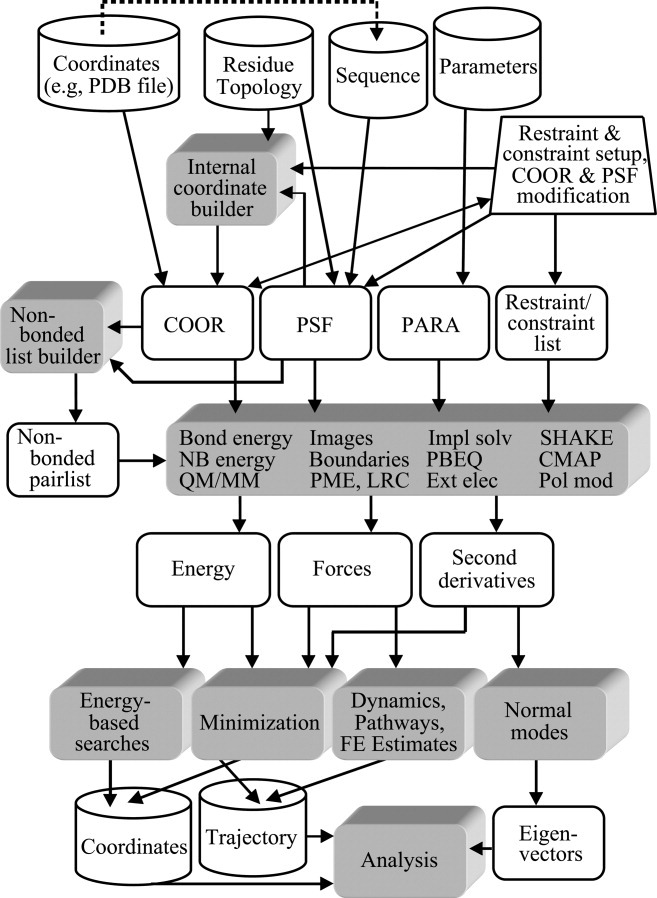
\includegraphics[width=0.6\textwidth]{images/charmm.jpg}
	\caption{Общая схема проекта CHARMM}
    \label{charmm}
\end{center}
\end{figure}


\section{Описание входных данных}


\subsection{Формат данных pdb}

Архив PDB представляет собой хранилище атомных координат и другой информации, описывающей белки и другие важные биологические макромолекулы. Структурные биологи используют такие методы, как рентгеновская кристаллография, ЯМР-спектроскопия и криоэлектронная микроскопия, чтобы определить положение каждого атома относительно друг друга в молекуле. Затем они размещают эту информацию, которая затем аннотируется и публикуется в архиве wwPDB.

Данные PDB
Первичная информация, хранящаяся в архиве PDB, состоит из файлов координат биологических молекул. В этих файлах перечислены атомы в каждом белке и их трехмерное расположение в пространстве. Эти файлы доступны в нескольких форматах (PDB, mmCIF, XML). Типичный файл в формате PDB включает в себя большой раздел <<заголовка>>, текста, в котором резюмируется белок, информация о цитировании и детали структурного решения, за которым следует последовательность и длинный список атомов и их координат. Архив также содержит экспериментальные наблюдения, которые используются для определения этих атомных координат.

Визуализация структур
Возможно просматривать файлы PDB напрямую с помощью текстового редактора, часто наиболее полезно использовать программу просмотра или визуализации для их просмотра. Онлайн-инструменты, такие как на веб-сайте RCSB PDB, позволяют искать и изучать информацию под заголовком PDB, включая информацию об экспериментальных методах, химии и биологии белка.

Потенциальные проблемы
При изучении архива PDB может возникуть ряд проблем. Например, многие структуры, особенно определяемые кристаллографией, включают информацию только о части функциональной биологической сборки. Кроме того, во многих записях PDB отсутствуют части молекулы, которые не наблюдались в эксперименте. К ним относятся структуры, включающие только положения альфа-углерода, структуры с отсутствующими петлями, структуры отдельных доменов или субъединиц более крупной молекулы. Кроме того, в большинстве записей кристаллографической структуры отсутствует информация об атомах водорода.

Центральным хранилищем данных о структуре биологических макромолекул является Protein Data Bank, доступный по адресу rcsb.org.

Уникальным идентификатором каждой структуры в Protein Data Bank является PDB ID. Данный идентификатор состоит из четырех символов, первый из которых, как правило, цифра; буквы в PDB ID принято писать заглавными, хотя большинство программ в данном случае не чувствительны к регистру символов. Примеры PDB ID: 4L9K, 1BTI, 2R33.

В файле данного формата каждая колонка обладает строго определенную длину и содержит определенную информацию:

\begin{itemize}
	\item 1-6 -- имя записи
	\item 7-11 -- серийный номер атома
	\item 13-16 -- имя атома
	\item 17 -- альтернативное имя атома
	\item 18-20 -- имя остатка
	\item 22 -- идентификатор цепи
	\item 23-26 -- номер остатка
	\item 27 -- код для вставки остатков
	\item 31-38 -- координата X атома
	\item 39-46 -- координата Y атома
	\item 47-54 -- координата Z атома
	\item 55-60 -- вместимость
	\item 61-66 -- температура
	\item 77-78 -- символ элемента
	\item 79-80 -- заряд атома
\end{itemize}

\subsection{Формат данных pqr}

Надежные модели электростатических взаимодействий важны для понимания событий раннего молекулярного распознавания, где доминируют дальнодействующие межмолекулярные взаимодействия и эффекты сольватации на биомолекулярные процессы. В то время как явные электростатические модели, которые рассматривают растворенное вещество и растворитель в атомарных деталях, являются общими, эти подходы обычно требуют тщательного уравновешивания и отбора проб для сведения интересующих свойств в интересующий статистический ансамбль. Континуальные подходы, которые интегрируют важные, но в значительной степени неинтересные степени свободы, жертвуют численной точностью в пользу надежной, но качественной точности и эффективности, устраняя необходимость отбора проб и уравновешивания, связанную с явными моделями растворов и растворителей.

Хотя существует выбор между несколькими моделями неявной сольватации, одна из самых популярных моделей неявной растворимости для биомолекул основана на уравнении Пуассона–Больцмана (ПБ). Уравнение ПБ обеспечивает глобальное решение для электростатического потенциала $\phi$ внутри и вокруг биомолекулы путем решения уравнения в частных производных

\begin{equation}
	\Delta \epsilon \Delta \phi - \sum_i^M c_i q_i e^{-\beta(q_i \phi + V_i)} = \rho
	\label{pde}
\end{equation}

Растворитель описывается объемной диэлектрической проницаемостью растворителя $\varepsilon_s$ и свойствами подвижных ионов $i = 1, ..., M$ описываемыми их зарядами $q_i$, концентрациями $c_i$ и стерическим потенциалом взаимодействия ионов с раствором $V_i$. Биомолекулярная структура включена в уравнение через $V_i$, функцию диэлектрического коэффициента и функцию распределения заряда $\rho$. Диэлектрическая проницаемость $\epsilon$ часто устанавливается равной постоянному значению $\varepsilon_{min}$ внутри молекулы и резко меняется на молекулярной границе до значения $\varepsilon_s$, которое описывает объем растворителя. Форма границы определяется размером и расположением атомов раствора, а также специфическими для модели параметрами, такими как характерный размер молекулы растворителя. Распределение заряда $\rho$ обычно представляет собой сумму дельта-распределений Дирака, расположенных в центрах атомов. Наконец, $\beta = {(5 \kappa T)}^{-1}$ — обратная тепловая энергия, где $\kappa$ -- постоянная Больцмана, а $T$ — температура. Потенциал $\phi$ может использоваться в различных приложениях, включая визуализацию, другие структурные анализы, моделирование диффузии и ряд других расчетов, требующих глобальных электростатических свойств. Теория ПБ является приближенной и, как следствие, имеет несколько хорошо известных ограничений, которые могут повлиять на ее точность, особенно для сильно заряженных систем или высоких концентраций солей. Несмотря на эти ограничения, методы ПБ по-прежнему очень важны и популярны для биомолекулярного структурного анализа, моделирования и симуляции.

Было разработано несколько пакетов программного обеспечения, которые решают уравнения Пуассона-Больцмана для оценки энергий, потенциалов и других свойств сольватации. Наиболее значимые (на основе пользовательской базы и цитирований) из них: CHARMM, AMBER, DelPhi, Jaguar, Zap, MIBPB и APBS. Тем не менее, APBS и связанный программный пакет PDB2PQR служат большому сообществу, насчитывающему около 27 000 пользователей, путем создания веб-серверов, связанных с веб-сайтом APBS, которые поддерживают подготовку биомолекулярных структур и быстрое решение методом конечных разностей. уравнения Пуассона–Больцмана, которые дополнены набором инструментов анализа. Большинство электростатических расчетов APBS следуют общему рабочему процессу, показанном на рисунке \ref{pdb2pqr}. Еще более широкий набор функций и более гибкая конфигурация доступны, когда APBS и PDB2PQR запускаются из командной строки на платформах Linux, Mac и Windows, и которые можно запускать локально или через веб-службы, предоставляемую разработанным NBCR набором инструментов Opal. Этот инструментарий позволяет переносить вычислительную нагрузку для научных приложений с интенсивным использованием процессора на удаленные вычислительные ресурсы, такие как ресурсы, предоставляемые Национальным ресурсом биомедицинских вычислений (NCBR). Наконец, APBS может работать с другими программами молекулярного моделирования, такими как AMBER, CHARMM, NAMD, Rosetta и TINKER. Общая поддержка интеграции APBS со сторонними программами обеспечивается библиотекой iAPBS.

Электростатические расчеты начинаются с определения структуры молекулы и параметров заряда и размера составляющих ее атомов. Составляющие атомы обычно группируются по типам со значениями заряда и размера, определяемыми типом атома в различных файлах силового поля, разработанных для неявных расчетов растворителя. APBS включает эту информацию в расчеты в формате <<PQR>>. PQR — это формат файла неизвестного происхождения, используемый несколькими программными пакетами, такими как MEAD и AutoDock. Файл PQR просто заменяет столбцы температуры и заполнения плоского файла PDB на заряд ператома $(Q)$ и радиус $(R)$. Существуют гораздо более элегантные способы реализации функциональности PQR с помощью более современных расширяемых форматов файлов, таких как mmCIF или PDBML; тем не менее, простой формат PDB по-прежнему является одним из наиболее широко используемых форматов, и поэтому дальнейшее использование формата PQR поддерживает широкую совместимость инструментов и рабочих процессов биомолекулярного моделирования. Программное обеспечение PDB2PQR является частью пакета APBS, который был разработан для помощи в преобразование файлов PDB в формат PQR. В частности, PDB2PQR автоматически настраивает, выполняет и оптимизирует структуру для расчетов электростатики Пуассона-Больцмана, выводя файл PQR, который можно использовать с APBS или другим программным обеспечением для моделирования.


\subsection{Тестовые данные}


Выполнение оценок разработанной оценочной функцией возможно только для полноатомных структур, представленных в формате PDB. Поскольку функция разрабатывалась для моделирования процесса образования комплекса кинетическим методом Монте-Карло, для проверки качества выполняемых оценок был сформирован набор тестовых комплексов, взятый из хранилища SKEMPI\cite{skempi}, представленный в работах~\cite{biom10071056, rate}. При этом из общего списка комплексов был выделен ограниченный набор структур. Исключены комплексы, содержащие разрывы в~главных цепях, а также комплексы, состоящие из трёх и более цепей. 

Набор наименований белков для тестового набора был получен из файлов топологии CHARMM.

Перед проведением численного эксперимента для всех комплексов проведена предварительная подготовка. С помощью пакета CHARMM выполнено восстановление структур в полноатомный вид, поскольку представленные в базе данных PDB структуры могут не включать определенные атомы. Затем средствами пакета CHARMM выполнена минимизация энергии. В результате для каждого комплекса формируются три стартовых PDB файла, для которых генерируются PQR файлы, содержащие частичные заряды для каждого атома. На последнем этапе производится оценка энергии средствами CHARMM и разработанной оценочной функцией. Сформированный список комплексов и начальных файлов (PDB и PQR) представлен в репозитории~\cite{vcs}.

Тестовый набор данных -- это белки 1TM1 и 1KXQ.